\documentclass{AsignaturaResumen}

\def\ISMAIN{1}
\SetTitulo{Ingeniería genética}
\setabbreviationstyle[acronym]{long-short}
\makeglossaries

    % Glosario

\newglossaryentry{polimorfismo}{
    name={Polimorfismo},
    description={Existencia de dos o más variantes (alelos) de una secuencia de ADN en una población}
}
\newglossaryentry{locus}{
    name={Locus},description={Posición que ocupa un gen en el cromosoma}}
\newglossaryentry{amplicones}{
    name={Amplicones},
    description={Secuencias de ADN producidas por la amplificación de la hebra original en una \acrshort{pcr}. Se identifican como las bandas de una electroforesis en gel}
}
\newglossaryentry{sucesion microbiana}{
    name={Sucesión microbiana},
    description={Evento donde las especies de microorganismos presentes en una muestran son reemplazadas por otras}
}
\newglossaryentry{variante de secuencia}{
    name={Variante de Secuencia de Amplicón},
    description={Amplicón único de un conjunto de secuencias obtenidas en una secuenciación ya corregida}
}
\newglossaryentry{homopolimero}{
    name={Homopolímero},
    description={Secuencia repetitiva de nucleótidos (AGTGCGAT\emph{AAAA}TGCAGT, p.e.)}
}

    % Acrónimos

\newacronym{si}{SI}{Sistema Internacional}
\newacronym{iubmb}{IUBMB}{Unión Internacional de Bioquímica y Biología Molecular}

\newacronym{ros}{ROS}{especies reactivas de oxígeno}

\newacronym{pb}{pb}{pares de bases}
\newacronym{kb}{kb}{kilobases}

\newacronym{adn}{ADN}{Ácido desoxirribonucléico}
\newacronym{adnc}{ADNc}{ADN complementario}
\newacronym{dntps}{dNTPs}{desoxirribonucleótidos trifosfato}
\newacronym{ddntps}{ddNTPs}{didesoxinucleótidos}

\newacronym{adnpol}{ADNpol}{ADN polimerasa}

\newacronym{pcr}{PCR}{Reacción en Cadena de la Polimerasa}
\newacronym{rapd}{RAPD}{ADN Polimórfico Amplificado al Azar}
\newacronym{rflp}{RFLP}{Fragmentos de Restricción de Longitud Polimórfica}
\newacronym{dpcr}{dPCR}{PCR digital}
\newacronym{ngs}{NGS}{Secuenciación de Nueva Generación}
\newacronym{smrt}{SMRT}{Secuenciación en Tiempo Real de Molécula Única}

\newacronym{ccs}{CCS}{Lecturas de Consenso Circular}
\newacronym{asv}{ASV}{Variante de Secuencia de Amplicón}

\newacronym{iqi}{IQI}{Índice de Calidad Infaunal}

\newacronym{sds}{SDS}{dodecilsulfato sódico}
\newacronym{dms}{DMS}{dimetilsulfato}
\newacronym{ctab}{CTAB}{bromuro de cetiltrimetilamonio}

\begin{document}

    \frontmatter

\Portada
\Indices

    \mainmatter


\part{Fundamentos de genética molecular}

    \chapter{Historia de la ingeniería genética} \input{01}
    \chapter{Principios generales} 
\section{Postulados de la ingeniería genética}

\begin{enumerate}
    \item Todas las propiedades de los seres vivos resultan de las propiedades de las proteínas que aquellos contienen.
    \item Las propiedades que posee una proteína dada resultan de la secuencia de aminoácidos que la conforman.
    \item La secuencia de aminoácidos de cada proteína está determinada por la secuencia de nucleótidos de los ácidos nucléicos
    \item Los ácidos nucléicos constituyen el material hereditario que cada organismo transmite a la siguiente generación.
\end{enumerate}

\part{Manipulación de ácidos nucléicos}

    \chapter{Enzimas nucleasas} \input{03}
    \chapter{Hibridación de ácidos nucléicos} 
La hibridación de ADN es el proceso mediante el cual dos cadenas de ADN o ARN se unen con secuencias complementarias mediante apareamiento de bases.

Algunos tipos son:

\begin{itemize}
    \item Northern blot, para ARN
    \item Southern blot, para ADN
    \item In Situ
    \item Hibridación fluorescente in situ (Fluorescent In Situ Hibridation o FISH)
    \item Microarreglos
\end{itemize}

\section{Desnaturalización}

Primero, se inicia separando las cadenas de ADN/ARN, esto mediante varios mecanismos, ya sea el aumento de temperatura, la inducción de cambios  en el pH o el uso de agentes químicos.

\section{Hibridación}

Luego se introducen las sondas complementarias. Estas sondas son fragmentos de ADN o ARN los cuales son diseñados para reconocer mediante complementariedad una secuencia específica de interés.

\section{Detección}

La detección se logra al marcar las sondas complementarias para luego medir tal marcaje. El marcaje de estas sondas puede realizarse con varios métodos, ya sean radioactivos, como el uso de Plomo 32 (\ce{^{32}P}), o no radioactivos, como la biotina la dioxigenina, el uso de fluoróforos o también enzimas-

\section{Stringencia}

Este parámetro mide el grado de rigurosidad de las condicines utilizadas para permitir o impedir la formación de híbridos imperfectamente complementarios. Un valor alto de strigencia indica mayor especificidad, mientras que unvalor bajo de strigencia refleja una menor especificidad

Este valor puede ser afectado por el manejo de la temperatura durante el proceso, la concentración de sales en la muestra, la longitud de la sonda complementaria, así como el contenido de Citosina/Guanina (CG) en el ADN de interés\footnote{La unión CG es más fuerte (3 puentes de hidrógeno) que la AT (2 puentes de hidrógeno), por lo que un mayor contenido de CG hace el paso la desnaturalización más dificil.}
    \chapter{Técnicas de amplificación de ácidos nucléicos} \ifx\ISMAIN\undefined
    \documentclass{AsignaturaResumen}
    \SetTitulo{Ingeniería genética}
    \setabbreviationstyle[acronym]{long-short}
\makeglossaries

    % Glosario

\newglossaryentry{polimorfismo}{
    name={Polimorfismo},
    description={Existencia de dos o más variantes (alelos) de una secuencia de ADN en una población}
}
\newglossaryentry{locus}{
    name={Locus},description={Posición que ocupa un gen en el cromosoma}}
\newglossaryentry{amplicones}{
    name={Amplicones},
    description={Secuencias de ADN producidas por la amplificación de la hebra original en una \acrshort{pcr}. Se identifican como las bandas de una electroforesis en gel}
}
\newglossaryentry{sucesion microbiana}{
    name={Sucesión microbiana},
    description={Evento donde las especies de microorganismos presentes en una muestran son reemplazadas por otras}
}
\newglossaryentry{variante de secuencia}{
    name={Variante de Secuencia de Amplicón},
    description={Amplicón único de un conjunto de secuencias obtenidas en una secuenciación ya corregida}
}
\newglossaryentry{homopolimero}{
    name={Homopolímero},
    description={Secuencia repetitiva de nucleótidos (AGTGCGAT\emph{AAAA}TGCAGT, p.e.)}
}

    % Acrónimos

\newacronym{si}{SI}{Sistema Internacional}
\newacronym{iubmb}{IUBMB}{Unión Internacional de Bioquímica y Biología Molecular}

\newacronym{ros}{ROS}{especies reactivas de oxígeno}

\newacronym{pb}{pb}{pares de bases}
\newacronym{kb}{kb}{kilobases}

\newacronym{adn}{ADN}{Ácido desoxirribonucléico}
\newacronym{adnc}{ADNc}{ADN complementario}
\newacronym{dntps}{dNTPs}{desoxirribonucleótidos trifosfato}
\newacronym{ddntps}{ddNTPs}{didesoxinucleótidos}

\newacronym{adnpol}{ADNpol}{ADN polimerasa}

\newacronym{pcr}{PCR}{Reacción en Cadena de la Polimerasa}
\newacronym{rapd}{RAPD}{ADN Polimórfico Amplificado al Azar}
\newacronym{rflp}{RFLP}{Fragmentos de Restricción de Longitud Polimórfica}
\newacronym{dpcr}{dPCR}{PCR digital}
\newacronym{ngs}{NGS}{Secuenciación de Nueva Generación}
\newacronym{smrt}{SMRT}{Secuenciación en Tiempo Real de Molécula Única}

\newacronym{ccs}{CCS}{Lecturas de Consenso Circular}
\newacronym{asv}{ASV}{Variante de Secuencia de Amplicón}

\newacronym{iqi}{IQI}{Índice de Calidad Infaunal}

\newacronym{sds}{SDS}{dodecilsulfato sódico}
\newacronym{dms}{DMS}{dimetilsulfato}
\newacronym{ctab}{CTAB}{bromuro de cetiltrimetilamonio}
    \begin{document}
    \chapter{Técnicas de amplificación de ácidos nucléicos}
\fi

\tikzset{
    primer paso/.style={draw, rounded corners=2pt, inner sep=1em, text width=3.5cm, align=center, font=\sffamily},
    paso/.style={primer paso, xshift=5.5cm},
    flecha/.style={-Stealth, ultra thick}
}


\section{Ensayos de amplificación: RAPD}

La técnica de \acrfull{rapd}\footnote{En inglés ``Random Amplified Polimorphic DNA''} es un método basado en la reacción en \acrshort{pcr} que permite la amplificación de ADN utilizando cebadores no específicos. Esta técnica fue desarrollada de forma independiente por \citet{williamsDNAPolymorphismsAmplified1990} y \citet{welshFingerprintingGenomesUsing1990}, y se utiliza para detectar la presencia de algún \gls{polimorfismo} en el ADN.

El fundamento del \acrshort{rapd} se basa en utilizar solamente un cebador de pocas \acrfull{pb}, generalmente alrededor de 10, a diferencia de una \acrshort{pcr} común donde los cebadores constan de aproximadamente 20\acrshort{pb}. Además, la secuencia de nucleótidos de estos cebadores no está diseñada para unirse a alguna secuencia dada, pues no se busca que amplifiquen una región específica del ADN, como si pasa con una \acrshort{pcr} común. Este par de características de los cebadores se combinan con condiciones de amplificación de baja stringencia, como temperaturas de entre \qtyrange{34}{36}{\degreeCelsius} en la etapa de hibridación. 

Las 3 condiciones anteriores lo que provocan es que se amplifiquen una gran cantidad de regiones, esto porque la corta longitud de los cebadores hace que, por mera probabilidad, se unan a muchas regiones a lo largo del ADN. Las amplificaciones resultantes tendrán una variedad dada de longitudes, algo así como un ``perfil de longitudes'', el cual se puede observar como las bandas resultantes en una electroforesis en gel. Así pues, la comparación de estos perfiles de tamaños permiten identificar diferencias entre los ADN de diferentes muestras, individuos, poblaciones, etc., esto dependiendo ya de con qué se esté trabajando \citep{kumariRandomlyAmplifiedPolymorphic2014, atienzarRandomAmplifiedPolymorphic2006}.

\resumebox{dato}{\acrshort{rapd} y diversidad microbiana}{\footnotesize
    Un estudio de 2013 ejemplifica el uso de la técnica \acrshort{rapd} en el estudio de diversidad microbiana de suelos. En este analizaron los suelos asociados a 3 plantas (\sci{Capparis decidua}, \sci{Calligonum polygonoides} y \sci{Cuminum cyminum}) del desierto de Thar, India.
    \\
    Siguiendo la técnica \acrshort{rapd}, encontraron un polimorfismo promedio de 86.7\%, esto concluido con solo identificar las diferencias entre los perfiles de tamaño en los geles. Se encontró también que 2 de las plantas (\sci{C. decidua} y \sci{C. polygonoides}) tenían resultados similares en sus grupos de muestras, indicando que posiblemente compartían especies de microorganismos entre sí. 
    \\
    Este artículo muestra como la técnica de \acrshort{rapd} es una técnica accesible y útil para la identificación de polimorfismos y, en este caso, viable para investigar la diversidad microbiana de un ambiente.
}


El objetivo principal de la técnica \acrshort{rapd} es la detección de polimorfismos en el ADN entre individuos, poblaciones o especies, lo cual permite la identificación de marcadores genéticos, todo esto sin requerir de información previa sobre el genoma analizado. Sus aplicaciones incluyen la identificación de variedades taxonómicas, el mapeo genético, el análisis de diversidad genética, la caracterización de patógenos y la detección de inestabilidad genómica en estudios de genotoxicidad y carcinogénesis \citep{kumariRandomlyAmplifiedPolymorphic2014, atienzarRandomAmplifiedPolymorphic2006}.

\begin{figure}
    \centering
    \resizebox{\linewidth}{!}{\begin{tikzpicture}
\node[primer paso] (extraccion) at (0,0) {Extracción de ADN};
\node[paso] (amplificacion) at (extraccion) {Amplificación con baja strigencia y primers no específicos};
\node[paso] (electroforesis) at (amplificacion) {Electroforesis en gel de agarosa};
\node[paso] (visualizacion) at (electroforesis) {Visualización con bromuro de etidio};
\node[paso] (analisis) at (visualizacion) {Comparación de bandas entre muestras};

\draw[flecha] (extraccion) -- (amplificacion);
\draw[flecha] (amplificacion) -- (electroforesis);
\draw[flecha] (electroforesis) -- (visualizacion);
\draw[flecha] (visualizacion) -- (analisis);

\node[primer paso, yshift=-4cm] (desnaturalizacion) at (amplificacion) {Desnaturalización};
\node[paso] (hibridacion) at (desnaturalizacion) {Hibridación:\\(A baja temperatura)};
\node[paso] (elongacion) at (hibridacion) {Elongación};

\draw[dashed, ultra thick] (amplificacion) -- (desnaturalizacion);
\draw[flecha] (desnaturalizacion) -- (hibridacion);
\draw[flecha] (hibridacion) -- (elongacion);
\draw[flecha] (elongacion.south) to[out=220,in=320] (desnaturalizacion.south);
\end{tikzpicture}}
    \rule{\linewidth}{0.5pt}
    \caption{Esquema metodológico de la técnica \acrshort{rapd}}
    \label{fig:esquema_de_rapd}
\end{figure}

El procedimiento general consta de los siguientes pasos \citep{kumariRandomlyAmplifiedPolymorphic2014}:

\begin{enumerate}
    \item \emph{Extracción de ADN}: Se aísla el ADN a partir de la muestra de interés mediante cualquier método estándar aplicable.
    \item \emph{Amplificación por \acrshort{pcr}}: El programa seguido es casi igual la seguido en una \acrshort{pcr} convencional: desnaturalización, hibridación y elongamiento. Esencialmente el único cambio es que se utilizan temperaturas más bajas en la etapa de hibridación, y van de \qtyrange{34}{36}{\degreeCelsius}. Esta baja temperatura es importante para permitir la unión del cebador a muchos sitios, incluso cuando se trate de un apareamiento imperfecto.
    \item \emph{Electroforesis y visualización}: Los productos de la \acrshort{pcr} se separan por tamaño mediante electroforesis en gel de agarosa. Las bandas de ADN se visualizan bajo luz ultravioleta utilizando un colorante, como lo puede ser el bromuro de etidio.
    \item \emph{Análisis de datos}: El patrón de bandas obtenido en el gel se documenta y compara entre muestras. La presencia o ausencia de bandas se utiliza para comparar la similitud genética entre muestras y encontrar aquellas que tengan polimorfismos.
\end{enumerate}

    \begin{table}
    \centering
    \caption{Lista de ventajas y desventajas de la técnica \acrshort{rapd}}
    \label{tab:ventajas_y_desventajas_rapd}
    {\tabstyle
    \begin{tabular}{m{0.45\linewidth}m{0.45\linewidth}}\hline 
         \theader{Ventajas} & \theader{Desventajas} \\ \hline
        
         No requiere conocimiento previo de la secuencia a estudiar
         &
         No se puede distinguir entre individuos homocigotos y heterocigotos 
         \\
         Es rápida, simple y de bajo costo
         &
         La reproducibilidad es delicada por la sensibilidad del patrón de la electroforesis
         \\
         Requiere poca cantidad de ADN por su alta sensibilidad
         &
         La interpretación de resultados es compleja, pues pueden existir varias razones para los cambios en las diferencias entre muestras
         \\
    \hline\end{tabular}}
\end{table}


% Falta: no mencionas la falta de reproducibilidad entre laboratorios como desventaja fuerte (sí la mencionas como "reproducibilidad delicada", pero podrías reforzarla).


    
    


\section{Ensayos de restricción: RFLP}

La técnica de \acrfull{rflp}, en inglés ``Restriction Fragment Length Polymorphism'', es un método que permite detectar diferencias en secuencias de ADN mediante el uso de enzimas de restricción para realizar ``cortes'' en el ADN y luego separar tales fragmentos en base a su tamaño. Los polimorfismos se detectan cuando la digestión genera fragmentos de diferentes longitudes entre muestras \citep{tarachApplicationPolymeraseChain2021}.

El fundamento de la técnica de \acrshort{rflp} inicia con las enzimas de restricción. Estas son un tipo de endonucleasas provenientes de bacterias y arqueas que tienen la capacidad de reconocer y cortar secuencias de ADN. Dentro de estas existen 4 tipos, siendo las Tipo II las más utilizadas por ser las más específicas \citep{tarachApplicationPolymeraseChain2021}.

La técnica de \acrshort{rflp} parte de la idea de que si se tiene un conjunto de muestras del mismo tipo o región de ADN y se les aplica un tratamiento con un grupo dado de enzimas de restricción, los cortes deberían darse en los mismos sitios en todas las muestras y, por ende, el conjunto de tamaños que tendrían los fragmentos obtenidos deberían ser iguales o muy similares entre las muestras. Tal ``perfil de tamaños'' de una muestra es obtenido mediante una electroforesis en gel (con agarosa o poliacrilamida) que es visualizado añadiendo bromuro de etidio o plata \citep{tarachApplicationPolymeraseChain2021}.

En caso de que una muestra de ADN tenga alguna o varias mutaciones a lo largo de su cadena, las enzimas de restricción cortarían en zonas diferentes, generando fragmentos de tamaños diferentes a los del resto de muestras. Es al comparar estos perfiles de tamaños en los geles de agarosa que la \acrshort{rflp} puede utilizarse para identificar la presencia de mutaciones en una muestra de ADN \citep{tarachApplicationPolymeraseChain2021,hashimExploringPotentialLimitations2019}.

\resumebox{dato}{\acrshort{rflp} en el estudio de microbiomas\citep{ikenagaCommunityStructureMicrobiota2002}}{\footnotesize
    Un estudio en 2002 analizó el cambio en las comunidades microbianas asociadas a las raíces de un cultivo de arroz siguiendo la metodología de \acrshort{rflp} (toma de muestra, extracción de \acrshort{adn}, digestión con enzimas de restricción y electroforesis). 
    \\
    Las diferencias en los perfiles de tamaños obtenidos en el gel permitieron identificar varios aspectos del microbioma estudiado, tales como un aumento en la diversidad microbiana con el paso del tiempo, la presencia de microorganismos característicos de diferentes etapas, así como indicios de \glsdisp{sucesion microbiana}{sucesiones microbianas} a lo largo de las etapas de crecimiento.
    \\
    Este estudio ejemplifica la utilidad de la \acrshort{rflp} en el contexto de estudios de ecología microbiana.
}

El objetivo del \acrshort{rflp} es detectar variaciones en la secuencia de ADN entre individuos, poblaciones o especies, con el fin de utilizarlas como marcadores genéticos \citep{tarachApplicationPolymeraseChain2021}. Las aplicaciones de la técnica incluyen la identificación de mutaciones, mapeo genético, estudios de diversidad genética, pruebas de paternidad y forenses, así como en el diagnóstico de enfermedades como la anemia falciforme \citep{tarachApplicationPolymeraseChain2021,hashimExploringPotentialLimitations2019}.

\begin{figure}
    \centering
    \resizebox{\linewidth}{!}{\begin{tikzpicture}
\node[primer paso] (extraccion) at (0,0) {Extracción de ADN};
\node[paso, dashed, ultra thick] (preamplificacion) at (extraccion) {Preamplificación\\(Situacional)};
\node[paso] (digestion) at (preamplificacion) {Digestión con enzimas de restricción};
\node[paso] (electroforesis) at (digestion) {Electroforesis en gel (agarosa o poliacrilamida)};
\node[paso] (visualizacion) at (electroforesis) {Visualización (bromuro de etidio o sondas)};
\node[paso] (analisis) at (visualizacion) {Comparación de bandas entre muestras};

\draw[flecha] (extraccion) -- (preamplificacion);
\draw[flecha] (preamplificacion) -- (digestion);
\draw[flecha] (digestion) -- (electroforesis);
\draw[flecha] (electroforesis) -- (visualizacion);
\draw[flecha] (visualizacion) -- (analisis);

\node[primer paso, yshift=-3cm] (desnaturalizacion) at (preamplificacion) {Desnaturalización};
\node[paso] (hibridacion) at (desnaturalizacion) {Hibridación};
\node[paso] (elongacion) at (hibridacion) {Elongación};

\draw[dashed, ultra thick] (preamplificacion) -- (desnaturalizacion);
\draw[flecha] (desnaturalizacion) -- (hibridacion);
\draw[flecha] (hibridacion) -- (elongacion);
\draw[flecha] (elongacion.south) to[out=220,in=320] (desnaturalizacion.south);
\end{tikzpicture}}
    \rule{\linewidth}{0.5pt}
    \caption{Esquema metodológico de la técnica \acrshort{rflp}}
    \label{fig:esquema_de_rflp}
\end{figure}

El procedimiento general consta de los siguientes pasos \citep{tarachApplicationPolymeraseChain2021}:

\begin{enumerate}
    \item \emph{Extracción de ADN}: Se aísla el ADN genómico de la muestra de interés.
    \item \emph{Preamplificación}: Este paso puede ser necesario para algunos tipos de estudios donde es necesario ``filtrar'' las muestras.
    \item \emph{Digestión con enzimas de restricción}: El ADN se incuba con una o más enzimas de restricción que reconocen secuencias específicas. La elección de la enzima depende del polimorfismo que se desea detectar.
    \item \emph{Electroforesis}: Los fragmentos de restricción resultantes se separan por tamaño mediante electroforesis en gel de agarosa o poliacrilamida.
    \item \emph{Visualización}: Los fragmentos se visualizan mediante tinción con bromuro de etidio para comparar los patrones de bandas entre muestras e identificar diferencias que indiquen polimorfismos, tales como bandas de diferentes tamaños o diferencias de presencia/ausencia de bandas entre muestras.
\end{enumerate}

    \begin{table}
    \centering
    \caption{Lista de ventajas y desventajas de la técnica \acrshort{rflp}}
    \label{tab:ventajas_y_desventajas_rflp}
    {\tabstyle
    \begin{tabular}{m{0.45\linewidth}m{0.45\linewidth}}\hline 
         \theader{Ventajas} & \theader{Desventajas} \\ \hline
        
         No requiere conocimiento previo de la secuencia para el análisis de mutaciones en \gls{locus} conocidos
         &
         Requiere grandes cantidades de ADN de alta calidad
         \\
         Alta especificidad y reproducibilidad
         &
         La digestión puede llegar a consumir mucho tiempo
         \\
         Permite distinguir homocigotos de heterocigotos
         &
         La digestión puede verse afectada por metilación del ADN o inhibidores
         \\
         Es una técnica de bajo costo en comparación con métodos de secuenciación
         &
         Limitada a la detección de polimorfismos en sitios de restricción
         \\
    \hline\end{tabular}}
\end{table}


    



\section{PCR Digital (dPCR)}

La \acrfull{dpcr}, en inglés ``Digital Polymerase Chain Reaction'', es una técnica que permite la cuantificación absoluta de ácidos nucleicos en una muestra. Esta técnica divide la muestra en una gran cantidad de microcompartimentos individuales de modo que, por estadística, cada uno contiene cero o unas pocas moléculas de la secuencia de interés. Tras la amplificación, la señal de fluorescencia se lee en cada compartimento y, mediante la distribución de Poisson, se calcula el número absoluto de copias en la muestra original \citep{maoPrinciplesDigitalPCR2019}.

\subsection{Fundamento}

El fundamento de la \acrshort{dpcr} se basa en la partición de la muestra. La mezcla de \acrshort{pcr} se divide en un gran número de compartimentos de volumen nanométrico, que pueden ser microcámaras en un chip o gotas de agua en aceite. Estas moléculas de ADN o ARN se distribuyen aleatoriamente entre ellos. Cada compartimento actúa como un microreactor independiente. Tras la amplificación, los compartimentos que contenían al menos una molécula diana emiten fluorescencia (se consideran positivos) y los que no, permanecen oscuros (negativos). La proporción de compartimentos positivos se utiliza para calcular la concentración inicial de la diana mediante la ley de Poisson, lo que permite una cuantificación absoluta sin necesidad de una curva de calibración \citep{maoPrinciplesDigitalPCR2019}.

Respecto a la estadística usada en la técnica, la Ley de Poisson se utiliza para calcular las probabilidades de que ocurran un número dado de eventos ($k$) en un intervalo dado, sea de espacio o tiempo. 

La fórmula general que se utiliza es la siguiente:

\begin{equation*}
    P(X=k) = \frac{e^{-\lambda} \cdot \lambda^{k}}{k!}
\end{equation*}  

Donde $k$ es el número de ocurrencias del evento y $\lambda$ es la tasa promedio de que ocurra tal evento. 

En el contexto de la \acrshort{dpcr}, $k$ sería el número de moléculas que son depositadas en cada compartimiento, mientras que $\lambda$ sería el número promedio de moléculas por compartimento. En la \acrshort{dpcr} no podemos determinar cuantas moléculas se depositan en cada compartimento, sin embargo, si podemos saber si en algún compartimento no se depositó ninguna, siendo este el caso de los compartimentos que no muestren amplificación después de la \acrshort{pcr}. Si tomamos esto en cuenta, podemos definir $k = 0$ y despejar la fórmula de la siguiente manera:

\begin{equation*}
    P(X=0)=\frac{e^{-\lambda}\cdot\lambda^{0}}{0!} \quad\longrightarrow\quad P(X=0)=\frac{e^{-\lambda}\cdot 1}{1} \quad\longrightarrow\quad P(X=0) = e^{-\lambda}
\end{equation*}

Asimismo, el término $P(X=0)$ representa la probabilidad de que compartimento no tenga ninguna molécula, y para obtenerlo basta con cuantificar qué porcentaje de compartimentos no mostraron amplificación, simplificando aún más la fórmula.

\begin{equation*}
    P(X=0) = \frac{N_{\text{Negativas (-)}}}{N_{\text{Total (T)}}} \quad\therefore\quad \frac{N^{-}}{N_{\text{T}}} = e^{-\lambda}
\end{equation*}

Con esto, solo necesitamos despejar $\lambda$ para tener la fórmula que nos permite saber cuál es la cantidad de ADN promedio por compartimento, esto únicamente en base a cuantificar cuantos compartimentos no amplificaron.

\begin{equation*}
    \frac{N^{-}}{N_{\text{T}}} = e^{-\lambda}
    \quad\longrightarrow\quad
    \ln\left(\frac{N^{-}}{N_{\text{T}}}\right) = -\lambda
    \quad\longrightarrow\quad
    \lambda = -\ln\left(\frac{N^{-}}{N_{\text{T}}}\right)
    \quad\longrightarrow\quad
    \lambda = \ln\left(\frac{N_{\text{T}}}{N^{-}}\right)
\end{equation*}

Por último, para conocer la concentración de ADN en la muestra completa ($C$) solo necesitamos dividir $\lambda$ entre el volumen de los compartimentos generados ($V$).

\begin{equation}\label{eq:cuantificacion_por_dpcr}
    C = \frac{\lambda}{V_{\text{Celda}}}
\end{equation}


\subsection{Objetivo de la técnica}

El objetivo principal de la \acrshort{dpcr} es la cuantificación absoluta y de alta precisión de un ADN dado en una muestra. Se utiliza para cuantificación de cargas virales, la detección de mutaciones raras en ADN, el diagnóstico prenatal no invasivo de algunas enfermedades, y el control de calidad en bibliotecas de \acrfull{ngs} \citep{maoPrinciplesDigitalPCR2019}. Es posible usarla también para monitoreo de técnicas de bioremediación \citep{caoDigitalPCREmerging2020}

\subsection{Metodología de la técnica}

\begin{figure}[H]
    \centering
    \resizebox{\linewidth}{!}{\begin{tikzpicture}
\node[primer paso] (extraccion) at (0,0) {Extracción de ADN};
\node[paso] (preparacion) at (extraccion) {Preparación de muestra a amplificar};
\node[paso] (division) at (preparacion) {División en una gran cantidad de microcompartimientos};
\node[paso, dashed, ultra thick] (amplificacion) at (division) {Amplificación};
\node[paso] (cuantificacion) at (amplificacion) {Cuantificación y cálculo de ADN en muestra};

\draw[flecha] (extraccion) -- (preparacion);
\draw[flecha] (preparacion) -- (division);
\draw[flecha] (division) -- (amplificacion);
\draw[flecha] (amplificacion) -- (cuantificacion);

\node[primer paso, yshift=-3cm] (desnaturalizacion) at (amplificacion) {Desnaturalización};
\node[paso] (hibridacion) at (desnaturalizacion) {Hibridación};
\node[paso] (elongacion) at (hibridacion) {Elongación};

\draw[dashed, ultra thick] (amplificacion) -- (desnaturalizacion);
\draw[flecha] (desnaturalizacion) -- (hibridacion);
\draw[flecha] (hibridacion) -- (elongacion);
\draw[flecha] (elongacion.south) to[out=220,in=320] (desnaturalizacion.south);
\end{tikzpicture}}
    \rule{\linewidth}{0.5pt}
    \caption{Esquema metodológico de la técnica \acrshort{dpcr}}
    \label{fig}:
\end{figure}

El procedimiento general consta de los siguientes pasos \citep{maoPrinciplesDigitalPCR2019}:

\begin{enumerate}
    \item \emph{Preparación de la muestra}: Se prepara la mezcla de reacción de \acrshort{pcr} de manera similar a la convencional (ADN/ARN molde, primers, sondas fluorescentes, \acrshort{adnpol} y \acrshort{dntps}).
    \item \emph{Particionamiento}: La mezcla se divide en miles de microcompartimentos, ya sea mediante un chip de microfluidos (\acrshort{dpcr} de chip) o mediante la generación de gotas de agua en aceite (\acrshort{dpcr} de gota).
    \item \emph{Amplificación por \acrshort{pcr}}: Los compartimentos se someten a ciclos térmicos para la amplificación del ADN. Cada compartimento actúa como un microreactor independiente.
    \item \emph{Lectura de fluorescencia}: Se mide la señal de fluorescencia en cada compartimento. Los compartimentos se consideran positivos (1) o negativos (0) en base a si amplificaron o no, respectivamente.
    \item \emph{Cuantificación absoluta}: El número de copias se calcula a partir de la proporción de compartimentos positivos/negativos mediante la distribución de Poisson (\autoref{eq:cuantificacion_por_dpcr}), obteniendo la concentración absoluta de la diana en la muestra original.
\end{enumerate}

\subsection{Ventajas y desventajas}

\begin{table}[H]
    \centering
    \caption{Lista de ventajas y desventajas de la técnica \acrshort{dpcr}}
    
    {\tabstyle
    \begin{tabular}{m{0.45\linewidth}m{0.45\linewidth}}\hline 
         \theader{Ventajas} & \theader{Desventajas} \\ \hline
        
         Cuantificación absoluta sin necesidad de curva de calibración
         &
         Rango dinámico estrecho en comparación con la \acrshort{pcr} en tiempo real
         \\
         Alta sensibilidad, precisión y tolerancia a inhibidores de la \acrshort{pcr}
         &
         Costo elevado de los equipos y reactivos
         \\
         Alta repetibilidad y precisión en los resultados
         &
         No permite la detección de múltiples dianas en un solo compartimento (multiplexación limitada)
         \\
         Requiere poca cantidad de muestra
         &
         La partición puede introducir errores en muestras de bajo número de copias
         \\
    \hline\end{tabular}}
\end{table}

\subsection{Ejemplo de aplicación: Análisis de bioindicadores en granjas de salmón \citep{oladiDigitalPCRAssays2026}}

Un ejemplo del uso de la \acrshort{dpcr} es el estudio de \citet{oladiDigitalPCRAssays2026}, quienes utilizaron \acrshort{dpcr} para cuantificar de manera precisa la presencia de ciertos identificadores de bacterias clave en sedimentos de granjas de salmón, esto para analizar si tal técnica sirve como bioindicador para determinar la salud del ecosistema.

Los investigadores tomaron muestras de sedimento de diferentes puntos de las granjas de salmón, cada uno con diferente \acrfull{iqi}\footnote{Corresponde a un tipo de indicador de salud ambiental}, para luego extraer el ADN con kits de extracción\footnote{Presuntamente DNeasy PowerSoil Kit}.  Los primers de la \acrshort{dpcr} fueron realizados a partir de ciertos \gls{variante de secuencia} (\acrshort{asv}) que ya estaban relacionados taxonómicamente con las bacterias \sci{Sulfurovum spp.}, \sci{Cytophaga spp.} y la familia \sci{Desulfuromonadaceae}. Así, la \acrshort{dpcr} lo que cuantificó fueron las copias de los 3 \acrshort{asv} y, de manera indirecta a partir de esto, se concluye la población de cada una de las bacterias.

La \acrshort{dpcr} fue realizada con un MasterMix, los primers anteriormente preparados y el ADN de la muestra. Esta preparación se sometió a un ciclo inicial de a \qty{95}{\degreeCelsius} durante \qty{2}{\min}, seguido de 40 ciclos de: desnaturalización a \qty{95}{\degreeCelsius} durante \qty{15}{\s}, hibridación a \qty{58.5}{\degreeCelsius} durante \qty{15}{\s}, y elongación a \qty{72}{\degreeCelsius} durante \qty{15}{\s}. Por último, se realizó un enfriamiento final a \qty{40}{\degreeCelsius} durante \qty{5}{\min}. Los resultados de la amplificación fueron cuantificados mediante la medición de la fluorescencia en las muestras, mientras que las concentraciones fueron calculadas con la relación de positivos/negativos y estadística de Poisson. 

Al comparar los resultados de la \acrshort{dpcr} con el \acrshort{iqi} de cada punto de muestreo, se encontró que la cantidad de copias de cada \acrshort{asv} era coherente con las características de la bacteria a la que estaba relacionado.

Los resultados del estudio son válidos para avanzar en la implementación del uso de \acrshort{asv} como bioindicadores, esto porque la precisión de cuantificación de la \acrshort{dpcr} es lo suficientemente potente para calcular de manera confiable una correlación entre \acrshort{asv} e índices ambientales que valide estos primeros como bioindicadores. 




% ---------------------------------------------------------------------------------------------------------------------------------- %

\clearpage\section[Secuenciación]{Secuenciación: De primera a cuarta generación} % Equipo de Gemma

% Introducción general
Las técnicas de secuenciación de ADN engloban el conjunto de métodos que permiten determinar el orden exacto de nucleótidos (A, C, G, T) en una molécula de ADN. Desde los primeros métodos manuales desarrollados a finales de los años 70, hasta las tecnologías masivas actuales, la secuenciación ha pasado por varias generaciones, cada una con mejoras en aspectos como la velocidad, costo, precisión y longitud de lectura. Cada uno de estos avances ha ayudado a revolucionar una gran cantidad de áreas científicas, tales como la genómica, el diagnóstico de enfermedades, la biología evolutiva y la biotecnología \citep{erenDNASequencingMethods2022}.

\subsection{Objetivo general de la técnica}

El objetivo de la secuenciación es determinar la secuencia de nucleótidos de un ácido nucleico, ya sea ADN o ARN. Esto es de utilidad para una gran cantidad de técnicas posteriores, tales como identificar genes, detectar mutaciones, estudiar la expresión de los genes en un individuo, caracterizar genomas, analizar la diversidad microbiana en un entorno, o llevar a cabo diagnósticos moleculares \citep{erenDNASequencingMethods2022}.

\bigskip

A continuación se realiza un recorrido por las diferentes generaciones que han tenido las técnicas de secuenciación genética, explicando en cada una el fundamento y la metodología general de algunas de las técnicas que conforman cada generación.



\subsection{Primera generación: Maxam-Gilbert y Sanger}

La primera generación de secuenciación comprende dos métodos desarrollados a finales de los años 70: el método de Maxam-Gilbert y el método de Sanger. Ambos se basan en realizar una preamplificación del ADN molde para luego realizar fragmentos a partir de este, esto mediante degradación química en el caso de Maxam y por terminación de cadena en el caso de Sanger. Las metodologías buscan generar fragmentos cuyo tamaño sea representativo de la secuencia de la cadena, de forma que sea posible descifrarle viendo los pesos de los fragmentos mediante una electroforesis en gel \citep{erenDNASequencingMethods2022}.


\subsubsection{Maxam-Gilbert}

\begin{figure}\centering
    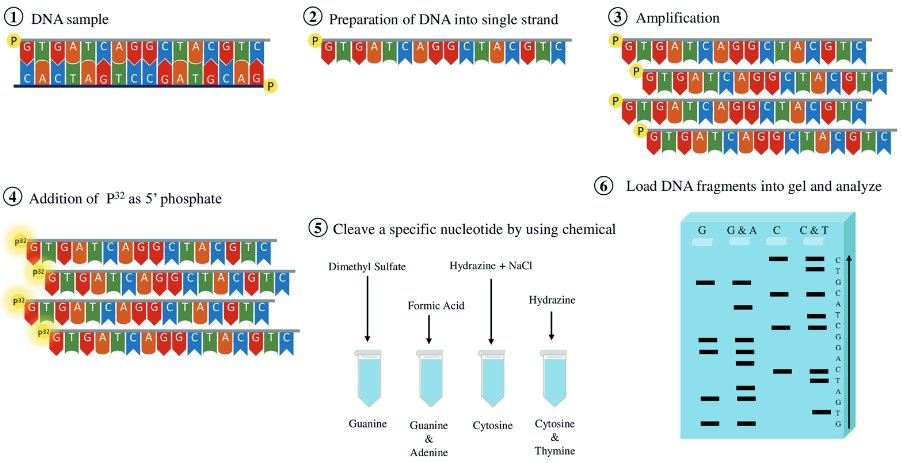
\includegraphics[width=\linewidth]{images/fig:secuenciacion_1g_maxam}
    \rule{\linewidth}{0.5pt}
    \caption{Representación gráfica de la metodología seguida en la técnica de secuenciación Maxam-Gilbert. La amplificación marcada es situacional. Extraído de \citet{erenDNASequencingMethods2022}}
    \label{fig:secuenciacion_1g_maxam}
\end{figure}

El método de Maxam-Gilbert se fundamenta en el uso de agentes químicos que cuentan con la capacidad de degradar el ADN de manera selectiva. Estos cortes precisos, junto con ciertas condiciones de reacción, hacen que los cortes generen fragmentos representativos de la secuencia de nucleótidos de la cadena muestra, los cuales pueden ser cuantificados mediante marcadores radioactivos y electroforesis.

Los siguientes agentes químicos (o agentes de marcado) actúan sobre algun nucleótido específico (o combinación de estos) de la forma en que se describe a continuación:

\begin{itemize}
    \item El \acrfull{dms} actua sobre la guanina, realizando una metilación (G)
    \item El ácido fórmico al igual que la anterior, realiza una metilación, pero en este caso en las zonas donde una adenina y guanina se unan (A+G)
    \item La hidracina en combinación con \ce{NaCl} actua sobre la citosina (C)
    \item La hidracina sin la presencia de \ce{NaCl} actua sobre las zonas de unión entre citosina y timina (C+T)
\end{itemize}

Para cada tipo de nucleótido (G, A+G, C, C+T) se realiza una reacción independiente, donde cada uno de estos agentes se encargará de marcar los nucleótidos correspondientes en la muestra. Para poder romper tales sitios marcados se utiliza piperidina, que se encarga de romper la cadena en aquellos lugares donde los 4 agentes anteriormente mencionados hayan actuado. Como último agente químico a comentar, es importante marcar el extremo $5^\prime$ con \ce{^{32}P} para poder realizar la electroforesis posterior.

El fundamento de esta técnica radica en que los agentes de marcado y la piperidina hacen que el ADN se corte en fragmentos de diferentes tamaños, entre estos, los fragmentos que nos importan son aquellos que parten del extremo $5^{\prime}$ marcado, pues son los que podrán ser visualizados en electroforesis. La electroforesis se realiza para cada reacción independiente, y al visualizar los tamaños de menor a mayor tamaño (de abajo hacia arriba) se puede inferir la secuencia original de la molécula de ADN.

Un detalle a tener en cuenta es que estos compuestos no están diseñados para detenerse una vez rompen la molécula de ADN de la forma en que nos interesa, por lo que para evitar que sigan actuando sobre los fragmentos marcados es importante hacer que la reacción dure poco y que los reactivos estén en concentraciones bajas, de no ser así, los reactivos degradarían las moléculas de ADN de interés a fragmentos que ya no son representativos de la secuencia original, imposibilitando la secuenciación.

\begin{figure}\centering
    \resizebox{\linewidth}{!}{\begin{tikzpicture}
\node[primer paso] (extraccion) at (0,0) {Extracción de ADN y separación de hebras individuales};
\node[paso] (preamplificacion) at (extraccion) {Preamplificación};
\node[paso] (marcaje) at (preamplificacion) {Marcaje del extremo $5^{\prime}$ (\ce{^{32}P})};
\node[paso] (digestion) at (marcaje) {Marcado de bases y corte con piperidina};
\node[paso] (electroforesis) at (digestion) {Electroforesis en gel de poliacrilamida};
\node[paso] (analisis) at (electroforesis) {Lectura de la secuencia};

\draw[flecha] (extraccion) -- (preamplificacion);
\draw[flecha] (preamplificacion) -- (marcaje);
\draw[flecha] (marcaje) -- (digestion);
\draw[flecha] (digestion) -- (electroforesis);
\draw[flecha] (electroforesis) -- (analisis);
\end{tikzpicture}}
    \rule{\linewidth}{0.5pt}
    \caption{Metodología general de la técnica de secuenciación de Maxam-Gilbert}
    \label{fig:secuenciacion_g1_maxam}
\end{figure}

Una metodología más general y resumida de esta técnica consistiría pues en lo siguiente: 

\begin{itemize}
    \item \emph{Marcaje radiactivo}: El ADN se marca con \ce{^{32}P} en el extremo $5^{\prime}$
    \item \emph{Separación de hebras}: Se desnaturaliza el ADN para obtener hebras simples
    \item \emph{Reacciones químicas específicas}: Se realizan cuatro reacciones independientes, una para cada nucleótido o combinación de tales
    \item \emph{Corte con piperidina}: La piperidina caliente rompe la cadena en los sitios marcados
    \item \emph{Electroforesis}: Los fragmentos se separan por tamaño en gel de poliacrilamida y se visualiza con rayos X
    \item \emph{Lectura de la secuencia}: El gel se lee de abajo hacia arriba, identificando la base cortada en cada carril
\end{itemize}

La técnica, como cualquier otra, presenta sus ventajas y desventajas (\autoref{tab:ventajas_desventajas_maxam}). Por varias de sus desventajas no suele ser tan utilizada hoy día.

\begin{table}\centering
    \caption{Lista de ventajas y desventajas de la técnica de secuenciación de Maxam-Gilbert}
    \label{tab:ventajas_desventajas_maxam}
    {\tabstyle
    \begin{tabular}{m{0.45\linewidth}m{0.45\linewidth}}\hline 
         \theader{Ventajas} & \theader{Desventajas} \\ \hline
        
         No requiere síntesis de ADN (útil para ADN con estructuras secundarias complejas)
         &
         Uso de químicos tóxicos y radiactividad
         \\
         Secuencia directamente el ADN original, sin amplificación previa
         &
         Laborioso y difícil de automatizar
         \\
         Útil para fragmentos cortos (hasta alrededor de 500\acrshort{pb})
         &
         Limitado a secuencias cortas
         \\
         No necesita cebadores ni polimerasa
         &
         Posibles errores en la lectura del gel, especialmente en regiones con bases repetidas
         \\\hline
\end{tabular}}\end{table}

\subsubsection{Sanger}

\begin{figure}[b]
    \begin{subfigure}[t]{0.485\linewidth}
        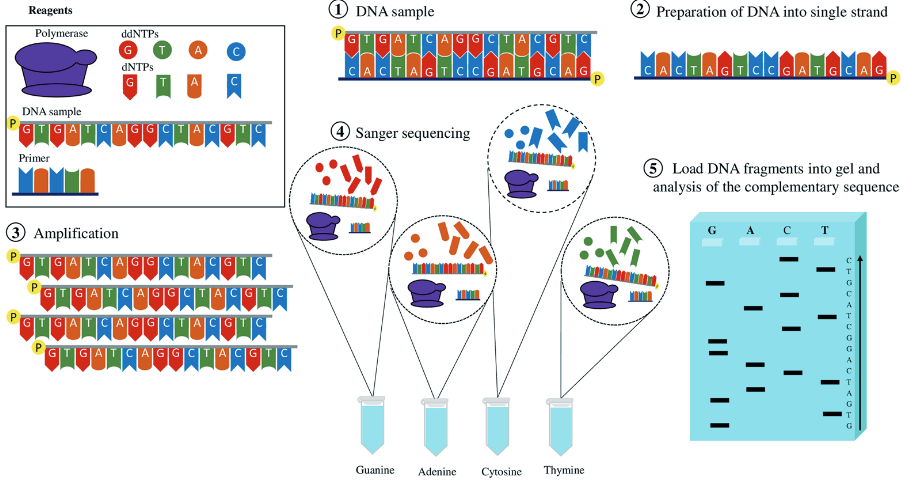
\includegraphics[width=\linewidth]{images/fig:secuenciacion_1g_sanger1}
        \caption{Técnica Sanger clásica}
        \label{fig:secuenciacion_1g_sanger1}
    \end{subfigure}
    \hfill
    \begin{subfigure}[t]{0.485\linewidth}
        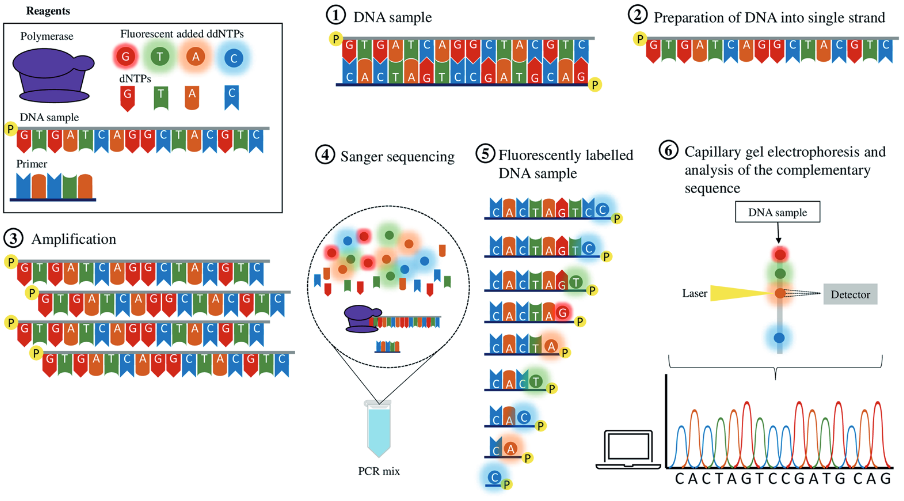
\includegraphics[width=\linewidth]{images/fig:secuenciacion_1g_sanger2}
        \caption{Técnica Sanger con fluorescencia}
        \label{fig:secuenciacion_1g_sanger2}
    \end{subfigure}
    
    \vspace*{10pt}
    \rule{\linewidth}{0.5pt}
    \caption{Representaciones gráficas de la metodologías seguidas en los dos tipos de método Sanger. Extraídos de \citet{erenDNASequencingMethods2022}}
\end{figure}

El método de Sanger, también llamado de terminación de cadena, utiliza un principio similar al de Maxam-Gilbert, sin embargo, mientras que el de Maxam utiliza un método ``destructivo'' al cortar el ADN en lugares clave, Sanger utiliza un principio ``constructivo'', pues se basa en crear la secuencia hasta un extremo dado para crear fragmentos que, al ser visualizados en electroforesis divididas por nucleótido, permite concluir la secuencia de nucleótidos del ADN original.

Esta detención de la elongación se logra al al agregar \acrfull{ddntps}, los cuales son nucleótidos especiales que carecen de grupo hidroxilo (\ce{OH}), lo que causa que cuando la \acrshort{adnpol} agrega uno de estos no pueda seguir avanzando, lo que detiene la elongación en tal punto.

El procedimiento de la técnica Sanger es similar a la de Maxam, pues ambos buscan obtener fragmentos que al visualizarlos en electroforesis (ambos procedimientos realizados por separado para cada nucleótido) permita visualizar el orden de nucleótidos en la secuencia original.

Con el tiempo, los \acrshort{ddntps} se marcaron con fluoróforos de distintos colores, permitiendo la reacción en un solo tubo y la automatización (\autoref{fig:secuenciacion_1g_sanger2}). De entre las dos formas de la técnica Sanger, esta que usa fluoróforos es el estándar \citep{erenDNASequencingMethods2022}.

\begin{figure}[H]\centering
    \resizebox{\linewidth}{!}{\begin{tikzpicture}
\node[primer paso] (extraccion) at (0,0) {Extracción de ADN};
\node[paso] (construccion) at (extraccion) {``Construcción'' de fragmentos (ddNTPs marcados)};
\node[paso] (electroforesis) at (construccion) {Electroforesis (capilar o en gel de poliacrilamida)};
\node[paso] (analisis) at (electroforesis) {Lectura de la secuencia};

\draw[flecha] (extraccion) -- (construccion);
\draw[flecha] (construccion) -- (electroforesis);
\draw[flecha] (electroforesis) -- (analisis);
\end{tikzpicture}}
    \rule{\linewidth}{0.5pt}
    \caption{Esquema metodológico de la técnica de secuenciación de Sanger}
    \label{fig:secuenciacion_g1_sanger}
\end{figure}

La metodología general de esta técnica es:

\begin{itemize}
    \item \emph{Amplificación (opcional)}: Se puede amplificar el ADN molde por PCR para obtener suficiente cantidad.
    \item \emph{Reacción de secuenciación}: Se mezcla el ADN molde con un cebador, una \acrlong{adnpol}, \acrshort{dntps} y \acrshort{ddntps} marcados con fluoróforos.
    \item \emph{Incorporación y terminación}: La polimerasa incorpora nucleótidos hasta que se añade un ddNTP, que termina la cadena.
    \item \emph{Electroforesis capilar}: Los fragmentos se separan por tamaño en un capilar.
    \item \emph{Detección de fluorescencia}: Un láser excita los fluoróforos y un detector captura la señal de cada fragmento.
    \item \emph{Lectura de la secuencia}: El orden de los picos de fluorescencia revela la secuencia.
\end{itemize}

\begin{table}[H]\centering
    \caption{Lista de ventajas y desventajas de la técnica de secuenciación de Sanger}
    {\tabstyle
    \begin{tabular}{m{0.45\linewidth}m{0.45\linewidth}}\hline 
         \theader{Ventajas} & \theader{Desventajas} \\ \hline
        
         Alta precisión y lectura larga (hasta 1000\acrshort{pb})
         &
         Bajo rendimiento (pocas secuencias a la vez)
         \\
         Estándar para validación de variantes
         &
         Costoso y lento para proyectos a gran escala
         \\
         Automatizable con fluoróforos y electroforesis capilar
         &
         Requiere cebadores específicos para cada región
         \\
         Ampliamente disponible y validado
         &
         No adecuado para secuenciación masiva
         \\\hline
\end{tabular}}\end{table}

\subsection{Segunda generación: Secuenciación masiva en paralelo (NGS)}

La segunda generación, también llamada \acrfull{ngs}, permite secuenciar millones de fragmentos simultáneamente. Se basa en la amplificación de fragmentos de ADN y en la detección de la incorporación de nucleótidos a estos. Diferentes compañías han creado plataformas (conjunto de tecnologías, instrumentos y herramientas) con tecnologías y fundamentos ligeramente diferentes. Las principales plataformas son: \emph{\nameref{sec:illumina}}, \emph{\nameref{sec:ion}}, \emph{\nameref{sec:roche_454}} y \emph{\nameref{sec:solid}} \citep{erenDNASequencingMethods2022}.

\subsubsection{Illumina}\label{sec:illumina}

La secuenciación por síntesis (SBS) con terminadores reversibles utiliza \acrshort{dntps} marcados con fluoróforos y un grupo bloqueante en el extremo $3^{\prime}$. En cada ciclo se incorpora un solo nucleótido, se lava, se detecta la fluorescencia y se desbloquea el grupo $3^{\prime}$ para permitir el siguiente ciclo. Es la plataforma más utilizada por su alta precisión y rendimiento \citep{erenDNASequencingMethods2022}.

\begin{figure}[H]\centering
    \resizebox{\linewidth}{!}{\begin{tikzpicture}
\node[primer paso] (extraccion) at (0,0) {Extracción de ADN};
\node[paso] (fragmentacion) at (extraccion) {Fragmentación del ADN};
\node[paso] (adaptadores) at (fragmentacion) {Ligación de adaptadores};
\node[paso] (flowcell) at (adaptadores) {Hibridación en celda de flujo};
\node[paso] (puente) at (flowcell) {Amplificación};
\node[paso] (sbs) at (puente) {Secuenciación por síntesis con terminadores reversibles};
\node[paso] (analisis) at (sbs) {Detección de fluorescencia y lectura de la secuencia};

\draw[flecha] (extraccion) -- (fragmentacion);
\draw[flecha] (fragmentacion) -- (adaptadores);
\draw[flecha] (adaptadores) -- (flowcell);
\draw[flecha] (flowcell) -- (puente);
\draw[flecha] (puente) -- (sbs);
\draw[flecha] (sbs) -- (analisis);
\end{tikzpicture}}
    \rule{\linewidth}{0.5pt}
    \caption{Esquema metodológico de la técnica de secuenciación Illumina}
    \label{fig:secuenciacion_g2_illumina}
\end{figure}

La metodología general de esta técnica es:

\begin{itemize}
    \item \emph{Fragmentación}: El ADN se fragmenta en trozos de 150-300\acrshort{pb}
    \item \emph{Ligación de adaptadores}: Se añaden adaptadores a los extremos de las cadenas
    \item \emph{Hibridación en celda de flujo}: La biblioteca se carga en una celda de flujo recubierta de oligonucleótidos complementarios a los adaptadores
    \item \emph{Amplificación}: Cada fragmento se amplifica formando grupos de millones de copias idénticas en un área pequeña
    \item \emph{Secuenciación por síntesis}: Se añaden \acrshort{dntps} terminadores reversibles marcados con fluoróforos. En cada ciclo se incorpora un solo nucleótido, se lava, se detecta la fluorescencia y se desbloquea el grupo $3^{\prime}$
    \item \emph{Lectura de la secuencia}: Las imágenes de fluorescencia de cada ciclo se procesan para identificar la base incorporada en cada grupo
\end{itemize}

\begin{table}[H]\centering
    \caption{Lista de ventajas y desventajas de la técnica de secuenciación Illumina}
    {\tabstyle
    \begin{tabular}{m{0.45\linewidth}m{0.45\linewidth}}\hline 
         \theader{Ventajas} & \theader{Desventajas} \\ \hline
        
         Altísima precisión (0.1\% de error)
         &
         Lecturas cortas (150-300 pb), lo que dificulta el ensamblaje de genomas complejos
         \\
         Altísimo rendimiento (miles de millones de lecturas por run)
         &
         Requiere amplificación por puente, lo que introduce sesgos
         \\
         Costo por base muy bajo
         &
         Tiempo de run variable (horas a días según el equipo)
         \\
         Versatilidad de equipos (MiSeq, HiSeq, NovaSeq)
         &
         Costo inicial del equipo elevado
         \\\hline
\end{tabular}}\end{table}

\subsubsection{Ion Torrent}\label{sec:ion}

La secuenciación por semiconductor detecta la liberación de protones (\ce{H+}) cuando se incorpora un nucleótido. El cambio de pH se mide con un sensor semiconductor, que lo convierte en una señal eléctrica. No requiere óptica, lo que reduce costos y tiempo \citep{erenDNASequencingMethods2022}.

\begin{figure}[H]\centering
    \resizebox{\linewidth}{!}{\begin{tikzpicture}
\node[primer paso] (extraccion) at (0,0) {Extracción de ADN};
\node[paso] (fragmentacion) at (extraccion) {Fragmentación del ADN};
\node[paso] (adaptadores) at (fragmentacion) {Ligación de adaptadores};
\node[paso] (emulsion) at (adaptadores) {PCR en microesferas};
\node[paso] (chip) at (emulsion) {Deposición en chip de semiconductor con micropocillos};
\node[paso] (protones) at (chip) {Secuenciación por detección de cambios de pH};
\node[paso] (analisis) at (protones) {Lectura de la secuencia};

\draw[flecha] (extraccion) -- (fragmentacion);
\draw[flecha] (fragmentacion) -- (adaptadores);
\draw[flecha] (adaptadores) -- (emulsion);
\draw[flecha] (emulsion) -- (chip);
\draw[flecha] (chip) -- (protones);
\draw[flecha] (protones) -- (analisis);
\end{tikzpicture}}
    \rule{\linewidth}{0.5pt}
    \caption{Esquema metodológico de la técnica de secuenciación Ion Torrent}
    \label{fig:secuenciacion_g2_ion}
\end{figure}

La metodología general de esta técnica es:

\begin{itemize}
    \item \emph{Fragmentación}: El ADN se fragmenta en trozos cortos
    \item \emph{Ligación de adaptadores}: Se añaden adaptadores a los extremos
    \item \emph{PCR en emulsión (emPCR)}: Los fragmentos se amplifican en microesferas
    \item \emph{Deposición en chip de semiconductor}: Las esferas se depositan en un chip con millones de micropocillos, cada uno con un sensor de pH
    \item \emph{Secuenciación por detección de protones}: Se añaden los \acrshort{dntps} uno por ciclo. Cuando se incorpora un nucleótido, se libera \ce{H+}, lo que cambia el pH y genera una señal eléctrica
    \item \emph{Lectura de la secuencia}: La señal eléctrica de cada pocillo en cada ciclo revela la base incorporada
\end{itemize}

\begin{table}[H]\centering
    \caption{Lista de ventajas y desventajas de la técnica de secuenciación Ion Torrent}
    {\tabstyle
    \begin{tabular}{m{0.45\linewidth}m{0.45\linewidth}}\hline 
         \theader{Ventajas} & \theader{Desventajas} \\ \hline
        
         No requiere óptica, lo que reduce costos y simplifica el equipo
         &
         Dificultad para leer \glsdisp{homopolimero}{homopolímeros} largos (similar a Roche 454)
         \\
         Rapidez (el cambio de pH es casi instantáneo)
         &
         Lecturas cortas (200-400\acrshort{pb})
         \\
         Equipos más económicos que Illumina
         &
         Menor rendimiento total que Illumina
         \\
         Buena para proyectos pequeños y de diagnóstico
         &
         Requiere \acrshort{pcr} en emulsión, con los sesgos asociados
         \\\hline
\end{tabular}}\end{table}

\subsubsection{Roche 454}\label{sec:roche_454}

La plataforma Roche 454 utiliza como base la pirosecuenciación, la cual es una técnica que se basa en sintetizar nucleótidos que, junto con otros reactivos y enzimas incluidos en el proceso, hacen que se libere luz cuando se une un nucleótido, lo cual se puede detectar con una cámara. Cada tipo de nucleótido se va añadiendo secuencialmente, o sea, uno por ciclo, lo que permite saber la secuencia del ADN. La altura del pico de medición es proporcional al número de nucleótidos incorporados \citep{erenDNASequencingMethods2022}.

\begin{figure}[H]\centering
    \resizebox{\linewidth}{!}{\begin{tikzpicture}
\node[primer paso] (extraccion) at (0,0) {Extracción de ADN};
\node[paso] (fragmentacion) at (extraccion) {Fragmentación del ADN};
\node[paso] (adaptadores) at (fragmentacion) {Ligación de adaptadores};
\node[paso] (emulsion) at (adaptadores) {PCR en microesferas};
\node[paso] (ptp) at (emulsion) {Deposición en placa de picotitulación};
\node[paso] (pirosecuenciacion) at (ptp) {Pirosecuenciación};
\node[paso] (analisis) at (pirosecuenciacion) {Lectura de la secuencia};

\draw[flecha] (extraccion) -- (fragmentacion);
\draw[flecha] (fragmentacion) -- (adaptadores);
\draw[flecha] (adaptadores) -- (emulsion);
\draw[flecha] (emulsion) -- (ptp);
\draw[flecha] (ptp) -- (pirosecuenciacion);
\draw[flecha] (pirosecuenciacion) -- (analisis);
\end{tikzpicture}}
    \rule{\linewidth}{0.5pt}
    \caption{Esquema metodológico de la técnica de secuenciación Roche 454}
    \label{fig:secuenciacion_g2_roche}
\end{figure}

La metodología general de esta técnica es:

\begin{itemize}
    \item \emph{Fragmentación}: El ADN se fragmenta para crear una ``biblioteca'' de trozos medianos (de 400-600\acrshort{pb})
    \item \emph{Emulsión}: La biblioteca se mezcla con microesferas y se diluye para que cada esfera capture alrededor de una molécula y los reactivos de PCR
    \item \emph{Depósito en placa}: Las esferas se depositan en una placa con pocillos, cada uno con una sola esfera
    \item \emph{Pirosecuenciación}: Se añaden secuencialmente los cuatro \acrshort{dntps} (uno por ciclo). Cuando se incorpora un nucleótido se libera luz que es captada por una cámara
    \item \emph{Lectura de secuencia}: El patrón de picos y la altura de cada pico en cada ciclo revela la secuencia del fragmento
\end{itemize}

\begin{table}[H]\centering
    \caption{Lista de ventajas y desventajas de la técnica de secuenciación Roche 454}
    {\tabstyle
    \begin{tabular}{m{0.45\linewidth}m{0.45\linewidth}}\hline 
         \theader{Ventajas} & \theader{Desventajas} \\ \hline
        
         Lecturas más largas (400-600\acrshort{pb}) que otras plataformas de segunda generación
         &
         Errores en \glsdisp{homopolimero}{homopolímeros} largos
         \\
         Detección de \glsdisp{homopolimero}{homopolímeros} mediante la altura del pico
         &
         Complejidad y riesgo de sesgos
         \\
         No requiere electroforesis
         &
         Costo por base elevado en comparación con Illumina
         \\\hline
\end{tabular}}\end{table}

\subsubsection{SOLiD}\label{sec:solid}

La secuenciación por ligación utiliza una ADN ligasa y sondas marcadas con fluoróforos. La lectura se basa en la ligación secuencial de sondas, no en la polimerización. Cada ciclo de ligación revela información sobre dos bases a la vez mediante un código de colores \citep{erenDNASequencingMethods2022}.

\begin{figure}[H]\centering
    \resizebox{\linewidth}{!}{\begin{tikzpicture}
\node[primer paso] (extraccion) at (0,0) {Extracción de ADN};
\node[paso] (fragmentacion) at (extraccion) {Fragmentación del ADN};
\node[paso] (adaptadores) at (fragmentacion) {Ligación de adaptadores};
\node[paso] (emulsion) at (adaptadores) {PCR en microesferas};
\node[paso] (flowcell) at (emulsion) {Deposición en celda de flujo};
\node[paso] (ligacion) at (flowcell) {Secuenciación por ligación (sondas marcadas)};
\node[paso] (analisis) at (ligacion) {Detección de fluorescencia y lectura de la secuencia};

\draw[flecha] (extraccion) -- (fragmentacion);
\draw[flecha] (fragmentacion) -- (adaptadores);
\draw[flecha] (adaptadores) -- (emulsion);
\draw[flecha] (emulsion) -- (flowcell);
\draw[flecha] (flowcell) -- (ligacion);
\draw[flecha] (ligacion) -- (analisis);
\end{tikzpicture}}
    \rule{\linewidth}{0.5pt}
    \caption{Esquema metodológico de la técnica de secuenciación SOLiD}
    \label{fig:secuenciacion_g2_solid}
\end{figure}

La metodología general de esta técnica es:

\begin{itemize}
    \item \emph{Fragmentación}: El ADN se fragmenta en trozos cortos.
    \item \emph{Ligación de adaptadores}: Se añaden adaptadores a los extremos.
    \item \emph{PCR en emulsión (emPCR)}: Los fragmentos se amplifican clonalmente en microesferas.
    \item \emph{Deposición en celda de flujo}: Las esferas se depositan en una celda de flujo.
    \item \emph{Secuenciación por ligación}: Se añaden sondas marcadas con fluoróforos. La ADN ligasa une la sonda complementaria a la secuencia. Cada ciclo de ligación revela información sobre dos bases mediante un código de colores. Tras varios ciclos, se deduce la secuencia.
    \item \emph{Lectura de la secuencia}: La combinación de colores de cada ciclo permite reconstruir la secuencia.
\end{itemize}

\begin{table}[H]\centering
    \caption{Lista de ventajas y desventajas de la técnica de secuenciación SOLiD}
    {\tabstyle
    \begin{tabular}{m{0.45\linewidth}m{0.45\linewidth}}\hline 
         \theader{Ventajas} & \theader{Desventajas} \\ \hline
        
         Alta precisión (99.85\% tras filtrado)
         &
         Lecturas muy cortas (50 pb)
         \\
         Buena para detección de variantes y RNA-seq
         &
         Proceso bioinformático complejo para interpretar el código de colores
         \\
         Rendimiento alto
         &
         Plataforma descontinuada por su complejidad y competencia con Illumina
         \\
         Menos errores en \glsdisp{homopolimero}{homopolímeros} que Roche 454
         &
         Requiere PCR en emulsión, con los sesgos asociados
         \\\hline
\end{tabular}}\end{table}



\subsection{Tercera generación: Secuenciación de molécula única en tiempo real}

La tercera generación, también llamada \textit{long-read sequencing}, permite secuenciar moléculas individuales de ADN sin amplificación por PCR, generando lecturas muy largas, de hasta decenas o cientos de miles de bases\footnote{Miles de pares de bases se denominan \acrfull{kb}}. Las plataformas principales son \nameref{sec:pacific} y \nameref{sec:oxford} \citep{erenDNASequencingMethods2022}.

\subsubsection{Pacific Bioscience (PacBio)}\label{sec:pacific}

La tecnología \acrfull{smrt}\footnote{En inglés ``Single Molecule Real-Time''} utiliza una polimerasa inmovilizada en el fondo de un pocillo nanométrico, y a medida que la polimerasa incorpora nucleótidos marcados con fluoróforos, se emite una señal luminosa que se detecta en tiempo real. El ADN de interés se puede  convertir en la molécula circular para que la polimerasa lo lea en repetidas ocasiones, generando algo llamado \acrfull{ccs}\footnote{En ingles ``Circular Consensus Sequencing''}, lo que que aumenta la precisión de la secuenciación \citep{erenDNASequencingMethods2022}.

\begin{figure}[H]\centering
    \resizebox{\linewidth}{!}{\begin{tikzpicture}
\node[primer paso] (extraccion) at (0,0) {Extracción de ADN};
\node[paso] (circularizacion) at (extraccion) {Circularización con adaptadores SMRTbell};
\node[paso] (zmw) at (circularizacion) {Inmovilización de polimerasa en pocillos ZMW};
\node[paso] (tiempo_real) at (zmw) {Secuenciación en tiempo real (dNTPs marcados)};
\node[paso] (deteccion) at (tiempo_real) {Detección de fluorescencia};
\node[paso] (ccs) at (deteccion) {Generación de lecturas de consenso circular (CCS)};
\node[paso] (analisis) at (ccs) {Lectura de la secuencia};

\draw[flecha] (extraccion) -- (circularizacion);
\draw[flecha] (circularizacion) -- (zmw);
\draw[flecha] (zmw) -- (tiempo_real);
\draw[flecha] (tiempo_real) -- (deteccion);
\draw[flecha] (deteccion) -- (ccs);
\draw[flecha] (ccs) -- (analisis);
\end{tikzpicture}}
    \rule{\linewidth}{0.5pt}
    \caption{Esquema metodológico de la técnica de secuenciación PacBio}
    \label{fig:secuenciacion_g3_pacific}
\end{figure}

La metodología general de esta técnica es:

\begin{itemize}
    \item \emph{Circularización}: El ADN se circulariza
    \item \emph{Inmovilización de la polimerasa}: Una polimerasa se inmoviliza en el fondo de un pocillo
    \item \emph{Secuenciación en tiempo real}: A medida que la polimerasa incorpora nucleótidos marcados con fluoróforos, se emite una señal luminosa que se detecta en tiempo real
    \item \emph{\acrfull{ccs}}: La polimerasa lee la misma molécula circular varias veces, generando \acrlong{ccs} que aumentan la precisión.
    \item \emph{Lectura de la secuencia}: La secuencia se deduce a partir de las señales luminosas de cada incorporación.
\end{itemize}

\begin{table}[H]\centering
    \caption{Lista de ventajas y desventajas de la técnica de secuenciación PacBio}
    {\tabstyle
    \begin{tabular}{m{0.45\linewidth}m{0.45\linewidth}}\hline 
         \theader{Ventajas} & \theader{Desventajas} \\ \hline
        
         Lecturas muy largas (10-100\acrshort{kb}), ideales para ensamblaje de genomas complejos
         &
         Mayor tasa de error por lectura individual (aunque mejorable con \acrshort{ccs})
         \\
         Sin amplificación por \acrshort{pcr}, lo que evita sesgos
         &
         Costo elevado del equipo y de los reactivos
         \\
         Detección de modificaciones epigenéticas de forma directa
         &
         Requiere mayor cantidad de ADN de alta calidad
         \\
         \acrlong{ccs} mejoran la precisión
         &
         Tiempo de procesado más largo que Illumina
         \\\hline
\end{tabular}}\end{table}

\subsubsection{Oxford Nanopore Technologies (ONT)}\label{sec:oxford}

Utiliza un nanoporo proteico insertado en una membrana que es a su vez atravesado por una corriente iónica. Cuando una hebra de ADN atraviesa el poro, cada base produce una interrupción característica de la corriente la cual puede ser interpretada por un algoritmo para determinar la secuencia. Esta técnica no requiere amplificación ni enzimas, y los equipos son incluso portátiles \citep{erenDNASequencingMethods2022}.

\begin{figure}[H]\centering
    \resizebox{\linewidth}{!}{\begin{tikzpicture}
\node[primer paso] (extraccion) at (0,0) {Extracción de ADN};
\node[paso] (adaptadores) at (extraccion) {Ligación de adaptadores (cola de poli-A y proteína motora)};
\node[paso] (nanoporo) at (adaptadores) {Inserción en nanoporo (membrana con corriente iónica)};
\node[paso] (translocacion) at (nanoporo) {Translocación de la hebra de ADN a través del nanoporo};
\node[paso] (corriente) at (translocacion) {Detección de cambios en la corriente iónica};
\node[paso] (algoritmo) at (corriente) {Interpretación algorítmica de la secuencia};
\node[paso] (analisis) at (algoritmo) {Lectura de la secuencia};

\draw[flecha] (extraccion) -- (adaptadores);
\draw[flecha] (adaptadores) -- (nanoporo);
\draw[flecha] (nanoporo) -- (translocacion);
\draw[flecha] (translocacion) -- (corriente);
\draw[flecha] (corriente) -- (algoritmo);
\draw[flecha] (algoritmo) -- (analisis);
\end{tikzpicture}}
    \rule{\linewidth}{0.5pt}
    \caption{Esquema metodológico de la técnica de secuenciación ONT}
    \label{fig:secuenciacion_g3_oxford}
\end{figure}

La metodología general de esta técnica es:

\begin{itemize}
    \item \emph{Ligación de adaptadores}: Se añade una proteína motora a los extremos del ADN
    \item \emph{Inserción en nanoporo}: El ADN se introduce en una membrana con un nanoporo proteico y una corriente iónica
    \item \emph{Translocación}: La proteína motora dirige la hebra de ADN a través del nanoporo
    \item \emph{Detección e interpretación de cambios en la corriente}: Cada base produce una interrupción característica en la corriente del poro que un algoritmo interpreta para determinar la secuencia
\end{itemize}

\begin{table}[H]\centering
    \caption{Lista de ventajas y desventajas de la técnica de secuenciación ONT}
    {\tabstyle
    \begin{tabular}{m{0.45\linewidth}m{0.45\linewidth}}\hline 
         \theader{Ventajas} & \theader{Desventajas} \\ \hline
        
         Lecturas ultra-largas (hasta cientos de \acrshort{kb})
         &
         Mayor tasa de error que Illumina (aunque mejorable con herramientas bioinformáticas)
         \\
         Sin amplificación ni enzimas, lo que evita sesgos
         &
         Bioinformática compleja para interpretar las señales
         \\
         Permite fabricar equipos portátiles
         &
         Requiere ADN de alta calidad y cantidad
         \\
         Detección directa de modificaciones epigenéticas
         &
         Menor rendimiento total que Illumina
         \\\hline
\end{tabular}}\end{table}

\subsection{Cuarta generación: Tecnologías emergentes}

La cuarta generación se refiere a tecnologías aún en desarrollo que buscan superar las limitaciones de las generaciones anteriores, como la secuenciación directa de ARN, la secuenciación de moléculas individuales sin nanoporos o el uso de nanotubos de carbono. No hay plataformas comerciales ampliamente establecidas, pero se espera que ofrezcan mayor precisión, portabilidad y menor costo \citep{erenDNASequencingMethods2022}.

Asimismo, no hay una metodología estandarizada, ya que las tecnologías están en fase de investigación. Se exploran aproximaciones como la secuenciación por nanotubos de carbono, la secuenciación directa de ARN sin conversión a \acrshort{adnc}, y otras que buscan eliminar la necesidad de amplificación y reducir el costo.




% ---------------------------------------------------------------------------------------------------------------------------------- %

\clearpage\section{Microarreglos} % Equipo de (Faltantes)

% Introducción rápida
Los microarreglos consisten en superficies sobre las cuales se inmovilizan miles de sondas de ADN en posiciones conocidas y ordenadas, donde cada posición del arreglo corresponde a una secuencia específica de interés, lo que permite analizar la presencia o abundancia de todas ellas al mismo tiempo \citep{jaksikMicroarrayExperimentsFactors2015, govindarajanMicroarrayItsApplications2012}.

\subsection{Fundamento}

Los microarreglos utilizan secuencias de ADN o ARN que son complementarias a la secuencia de interés (sondas) tal cómo otros métodos de \acrshort{pcr} utilizan. Sin embargo, lo particular sobre los microarreglos es que utilizan una cantidad enorme de compartimentos, cada uno con una sonda para una secuencia de interés dada, lo que permite analizar la expresión de una gran cantidad de secuencias a la vez \citep{govindarajanMicroarrayItsApplications2012,jaksikMicroarrayExperimentsFactors2015}.

Los microarreglos están construidos como portaobjetos de vidrio con compartimentos construidos en su superficie. Dentro de estos compartimentos las sondas se depositan, lo cual puede hacerse al construirlas ahí mismo (método \textit{in situ}) o depositadas. Un punto clave para el funcionamiento de la técnica es que se conoce la posición de cada sonda \citep{govindarajanMicroarrayItsApplications2012,jaksikMicroarrayExperimentsFactors2015}.

El método \textit{in situ} consiste en utiliza fotolitografía para construir las sondas dentro del compartimento. Este método parte por cubrir la superficie del compartimento con una capa de moléculas a la que los nucleotidos son afines, generalmente grupos hidroxilo (\ce{OH}). Además, a estos nucleotidos se les añade un grupo fotolábil\footnote{Moléculas que son sensibles a la luz y se degradan con esta}. La construcción de las sondas consiste en aplicar luz a través máscaras, lo que deja pasar la luz y, por ende, degradar los grupos fotolábiles, solo en ciertas regiones. Luego de dejar disponibles tales grupos se añade un tipo de nucleótido para que se una en esos espacios ``liberados'' en el paso anterior. En cada ``ciclo'' se liberan espacios determinados con la máscara y se añade un tipo de nucleótido. Para construir pues una sonda dada se sigue un patrón específico de ciclos  \citep{fodorLightDirectedSpatiallyAddressable1991}.

\begin{figure}\centering
    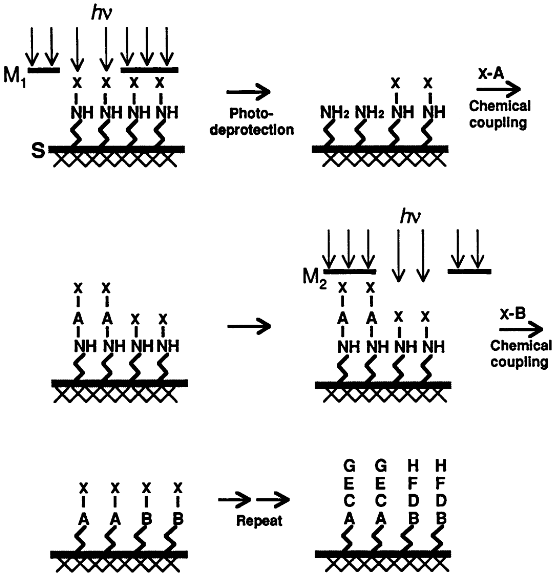
\includegraphics[width=0.5\linewidth]{images/fig:creacion_de_microarreglos_in_situ}
    \rule{\linewidth}{0.5pt}
    \caption{Generalización del proceso de construcción de sondas mediante fotolitografía (metodo \textit{in situ}). Extraído de \citet{fodorLightDirectedSpatiallyAddressable1991}}
\end{figure}

En el caso de ser depositadas, las sondas deben de ser inmovilizadas, esto utilizando alguno de los siguientes métodos \citep{nimseImmobilizationTechniquesMicroarray2014}:

\begin{itemize}
        \item \emph{Adsorción}: Las sondas se inmovilizan mediante interacciones no covalentes, como fuerzas electrostáticas o interacciones hidrofóbicas. Es el método más simple, pero las sondas quedan con una orientación aleatoria y pueden desprenderse con cambios de pH, fuerza iónica o detergentes, lo que afecta la reproducibilidad y la sensibilidad del arreglo.
    \item \emph{Inmovilización covalente}: Las sondas se unen a la superficie mediante enlaces químicos estables, generalmente con grupos funcionales amino o tiol. Este método proporciona una mayor estabilidad y fuerza de unión, y permite controlar mejor la orientación de las sondas, aunque requiere una modificación química previa de la superficie y de las sondas.
    \item \emph{Interacciones estreptavidina-biotina}: Se basa en la unión altamente específica y de gran afinidad entre la proteína estreptavidina, que se inmoviliza en la superficie del microarreglo, y la biotina, que se une a la sonda. Es un método que mejora la orientación y accesibilidad de las sondas, pero requiere múltiples etapas de preparación, es más costoso y puede sufrir problemas de estabilidad de las proteínas inmovilizadas. 
\end{itemize}

Antes de añadir la muestra a analizar, a esta se le añade un fluoróforo, esto con el fin de poder cuantificar su presencia al final. Una vez se añade la muestra al microarreglo, ocurre un sencillo proceso de hibridación donde las moléculas de ADN de la muestra se unirán a las sondas del microarreglo que sean complementarias. Una vez finalizado este proceso, el microarreglo se lava para eliminar las moléculas de ADN no hibridadas \citep{govindarajanMicroarrayItsApplications2012,jaksikMicroarrayExperimentsFactors2015}.

Dado que se conoce la sonda de cada compartimento, basta con medir la fluorescencia a lo largo de los compartimentos del microarreglo con un escáner para saber qué secuencias se encontraban en la muestra (presencia/ausencia de fluorescencia) y aproximar su cantidad (nivel de fluorescencia) \citep{govindarajanMicroarrayItsApplications2012,jaksikMicroarrayExperimentsFactors2015}.

\subsection{Objetivo de la técnica}

El objetivo principal de los microarreglos es el poder analizar miles de moléculas en una sola muestra, permitiendo obtener una gran cantidad de información en poco tiempo. Los procedimientos en los que se suele utilizar consisten en medir de perfiles de expresión génica, detectar polimorfismos y mutaciones, identificar de biomarcadores o caracterizar comunidades microbianas. Sus áreas de aplicación incluyen la investigación en cáncer, el diagnóstico molecular, la farmacogenómica y el monitoreo ambiental \citep{govindarajanMicroarrayItsApplications2012, jaksikMicroarrayExperimentsFactors2015}.

\subsection{Metodología general de la técnica}

\begin{figure}[H]
    \centering
    \resizebox{\linewidth}{!}{\begin{tikzpicture}
\node[primer paso] (extraccion) at (0,0) {Extracción de ADN};
\node[paso] (preparacion) at (extraccion) {Preparación de muestra a amplificar};
\node[paso] (marcaje) at (preparacion) {Marcaje con fluoróforos};
\node[paso] (deposito) at (marcaje) {Depósito de muestra en chip de amplificación};
\node[paso, dashed, ultra thick] (amplificacion) at (deposito) {Amplificación};
\node[paso] (lavado) at (amplificacion) {Lavado de secuencias no hibridadas};
\node[paso] (visualizacion) at (lavado) {Visualización y análisis de resultados};

\draw[flecha] (extraccion) -- (preparacion);
\draw[flecha] (preparacion) -- (marcaje);
\draw[flecha] (marcaje) -- (deposito);
\draw[flecha] (deposito) -- (amplificacion);
\draw[flecha] (amplificacion) -- (lavado);
\draw[flecha] (lavado) -- (visualizacion);

\node[primer paso, yshift=-3cm] (desnaturalizacion) at (amplificacion) {Desnaturalización};
\node[paso] (hibridacion) at (desnaturalizacion) {Hibridación};
\node[paso] (elongacion) at (hibridacion) {Elongación};

\draw[dashed, ultra thick] (amplificacion) -- (desnaturalizacion);
\draw[flecha] (desnaturalizacion) -- (hibridacion);
\draw[flecha] (hibridacion) -- (elongacion);
\draw[flecha] (elongacion.south) to[out=220,in=320] (desnaturalizacion.south);
\end{tikzpicture}}
    \rule{\linewidth}{0.5pt}
    \caption{Esquema metodológico de la técnica de microarreglos}
    \label{fig:esquema_de_microarreglos}
\end{figure}

El procedimiento general consta de los siguientes pasos \citep{jaksikMicroarrayExperimentsFactors2015}:

\begin{enumerate}
    \item \emph{Aislamiento y preparación del ácido nucleico}: Se extrae el ADN o ARN de la muestra, se evalúa su calidad e integridad y, en el caso del ARN, se convierte a \acrshort{adnc}. Además, se marca el material genético de la muestra con un fluoróforo.
    \item \emph{Hibridación}: La muestra marcada se pone en contacto con el arreglo y se incuba en condiciones que favorecen la hibridación específica entre las secuencias diana y las sondas inmovilizadas.
    \item \emph{Lavado}: Se elimina el material no hibridado mediante lavados con buffers.
    \item \emph{Visualización y análisis}: El microarreglo se escanea con un láser que excita los fluoróforos y un detector que mide la intensidad de fluorescencia en cada posición.
\end{enumerate}

\subsection{Ventajas y desventajas}

\begin{table}[H]
    \centering
    \caption{Lista de ventajas y desventajas de la técnica de microarreglos}
    \label{tab:microarreglos}
    {\tabstyle
    \begin{tabular}{m{0.45\linewidth}m{0.45\linewidth}}\hline 
        \theader{Ventajas} & \theader{Desventajas} \\ \hline
        
        Permite el análisis simultáneo de miles de genes o secuencias en una sola muestra
        &
        Alto costo de los equipos y reactivos
        \\
        Requiere poca cantidad de muestra
        &
        La precisión y especificidad pueden verse afectadas por hibridación no específica y por el diseño de las sondas
        \\
        Es una técnica rápida y de alto rendimiento
        &
        La interpretación de los datos es compleja y requiere métodos estadísticos sofisticados
        \\
        Permite la identificación de marcadores genéticos sin conocimiento previo de la secuencia
        &
        La sensibilidad a variaciones en las condiciones experimentales (temperatura, pureza del material, etc.) puede afectar la reproducibilidad
        \\
    \hline\end{tabular}}
\end{table}

\subsection{Ejemplo de aplicación: Expresión de genes en tomate expuesto a metales pesados \citep{houMicroarrayBasedAnalysisGene2015}}

El estudio de \citet{houMicroarrayBasedAnalysisGene2015} es un buen ejemplo del uso de microarreglos en el análisis de expresión génica en un organismo. Este equipo encontró que los análisis morfológicos en plantas (análisis de raíces, tallos y hojas) no terminaban de ser suficientes para analizar el impacto de metales pesados cuando estos estaban en cantidades muy pequeñas. Ante esto, analizaron la viabilidad de emplear microarreglos como método de detección de toxicidad de metales pesados a pequeñas concentraciones, además de permitir la identificación de los genes cuya expresión cambiaba.

Para la investigación se realizó un ensayo en el que se sometió a plántulas de tomate (\sci{Lycopersicon esculentum}) a concentraciones bajas de metales pesados (\ce{Cd}, \ce{Cr}, \ce{Hg} y \ce{Pb}). Posteriormente, se buscaron cambios morfológicos en las raíces (longitud, biomasa, contenido de malondialdehído, aminoácidos totales y viabilidad de la raíz), los cuales no mostraron diferencias significativas respecto al control, confirmando que los bioensayos convencionales no detectan el estrés temprano a esas concentraciones.

Para el análisis por microarreglos se utilizaron microarreglos de genoma completo de tomate de la empresa Agilent, y los protocolos de todos los procesos fueron proporcionados por el fabricante. Estos constaron de una extracción de ARN con TRIZOL\footnote{Fórmula comercial de fenol, tiocianatos y buffers utilizada para la extracción de ácidos nucleicos}, una conversión a \acrshort{adnc} y etiquetado con kits, un proceso de hibridación de 17 horas, un lavado con buffer del fabricante y adquisición de datos mediante un escáner especializado.

Los resultados mostraron que, aunque los análisis morfológicos no revelaron estrés, el análisis por microarreglos detectó cambios significativos en la expresión de numerosos genes: 252 genes para \ce{Cd}, 394 para \ce{Cr}, 605 para \ce{Hg} y 1366 para \ce{Pb} (\autoref{fig:microarreglos_ejemplo_cuantificacion_de_genes_por_tratamiento}). 

Además, se encontró que cada metal generaba cambios en diferentes conjuntos de genes (\autoref{fig:microarreglos_ejemplo_heatmap_de_expresion}), lo que es de utilidad para poder diferenciar el tipo de contaminante. 

Finalmente, se identificaron genes específicos de cada metal (29 para Cd, 58 para Cr, 192 para Hg y 864 para Pb) que podrían servir como biomarcadores potenciales. 

Los hallazgos de este estudio muestran que los microarreglos son potencialmente una herramienta viable para la detección temprana de toxicidad por metales pesados en suelos agrícolas, así como para la identificación del metal presente.

\ifx\ISMAIN\undefined
    \end{document}
\fi

\part{ADN recombinante}

    \chapter{Introducción al ADN recombinante} \input{06}
    \chapter{Construcción, clonación y selección de ADN} \input{07}
    \chapter{Mutagénesis dirigida} \input{08}



    \PlainGeom
    \appendix



    \backmatter
    
\Bibliografia
\Glosarios

\end{document}